\PassOptionsToPackage{english}{babel}
\documentclass{report}
\usepackage[utf8]{inputenc}

%\usepackage[english]{babel}
%\usepackage[latin1]{inputenc}
%\usepackage{geometry}
%\usepackage{listings}
\usepackage{caption}
\usepackage{amsmath}
\usepackage{graphics}
\usepackage[T1]{fontenc}
\usepackage{enumitem} %bold enumeration
\usepackage[utf8]{inputenc}
\usepackage[english]{babel}
%\usepackage{pmgraph}
\usepackage{mathrsfs}
\usepackage{floatflt}
\usepackage{multicol}
\usepackage{color,colortbl}
% \usepackage[pdftex]{graphicx}
\usepackage[normalem]{ulem}
\usepackage[colorlinks,urlcolor=blue, linkcolor=blue]{hyperref}
\usepackage{epstopdf}
\usepackage{wrapfig}
\usepackage{multirow}
%% Sets page size and margins
\usepackage[a4paper,top=3cm,bottom=2cm,left=3cm,right=3cm,marginparwidth=1.75cm]{geometry}
%% Useful packages
\usepackage[colorinlistoftodos]{todonotes}
\usepackage{xymtex}
\usepackage{fancyhdr}
\usepackage{epstopdf}
\usepackage{indentfirst} \geometry{verbose,a4paper,tmargin=3cm,bmargin=3cm,lmargin=1.0cm,rmargin=2.0cm}
\setlength{\parindent}{0pt}
\begin{document}
\large
Report of Anton Maksimov (antonma, 16-952-137), Task 9 "Shape from silhouettes"\\
 on ETHZ course "Computer Vision".\\
\rule{\linewidth}{1pt}
%%%%%%%%%%%%%%%%%%%%%%%%%%%%%%%%%%%%%%%%%%%%%%%%%%%%%%%%%   1
	\textbf{1.} Parameters used:\\
	
	\texttt{silhouetteThreshold = 110;}\\
	We chose this threshold to be low enough to include the whole statue even if there are some detected areas at the top and bottom of image, which are not in the bounding box and therefore won't be detected as statue later.\\
	
	\texttt{bbox = [0 0 -2; 3 3 2.5];}\\
	Box is small enough but includes the whole statue inside (with further refinements of its coordinates parts of statue start to disappear from the model)\\
	
	\texttt{volumeX = 64;}\\
	\texttt{volumeY = 64;}\\
	\texttt{volumeZ = 128;}\\ 
	and\\
	\texttt{volumeX = 128;}\\
	\texttt{volumeY = 128;}\\
	\texttt{volumeZ = 256;}\\ 
	
	\textbf{Details of implementation}\\
	In order to restrict projected centers of parallelepipeds in bounding box to correspond some pixel on the corresponding silhouette image, we round coordinates to the closest integer and then check that these rounded coordinates are inside the image (but $x$ coordinate of projection corresponds to $y$ of the silhouette image and vice versa).
	
	
	
		\begin{figure}[h]
		\begin{center}
			\label{tang1}
			\begin{minipage}[h]{0.95\linewidth}
				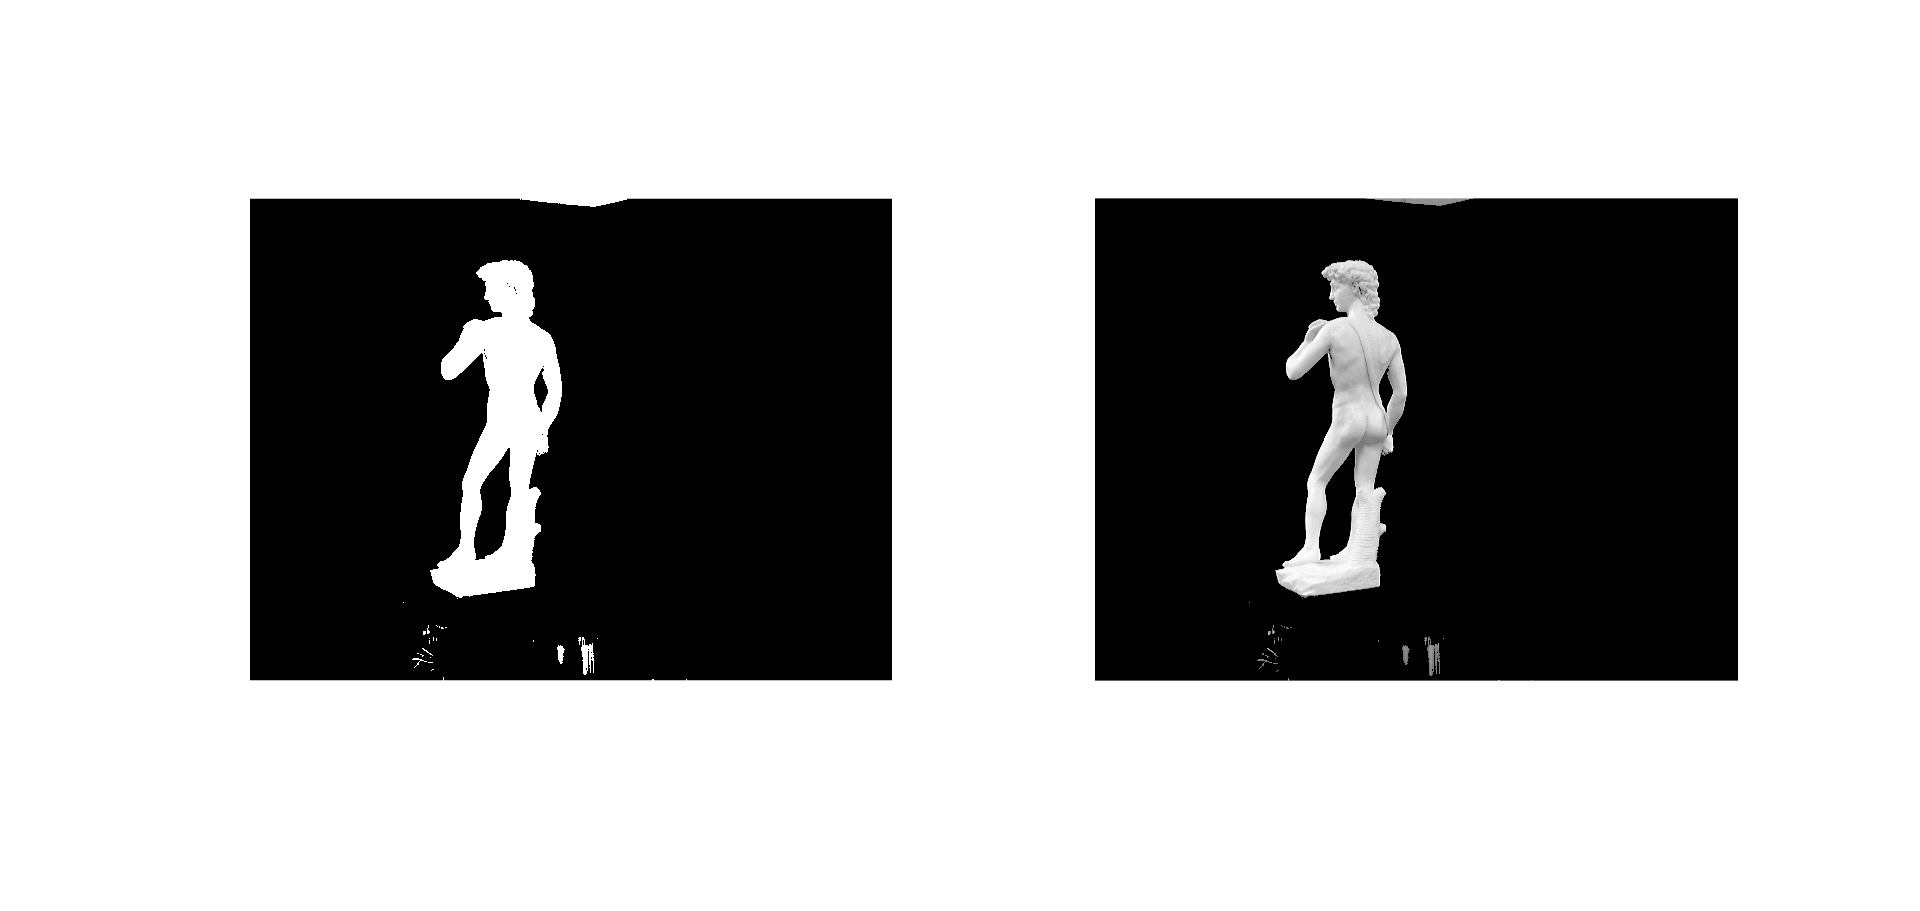
\includegraphics[width=1\linewidth, trim = {7cm 5cm 5cm 5cm}, clip]{C:/Users/Anton/Desktop/ETH_books/CV/cv_lab09_shape_from_silhouettes/code/results/untitled2}
			\end{minipage}
			\vfill
			\begin{minipage}[h]{0.95\linewidth}
				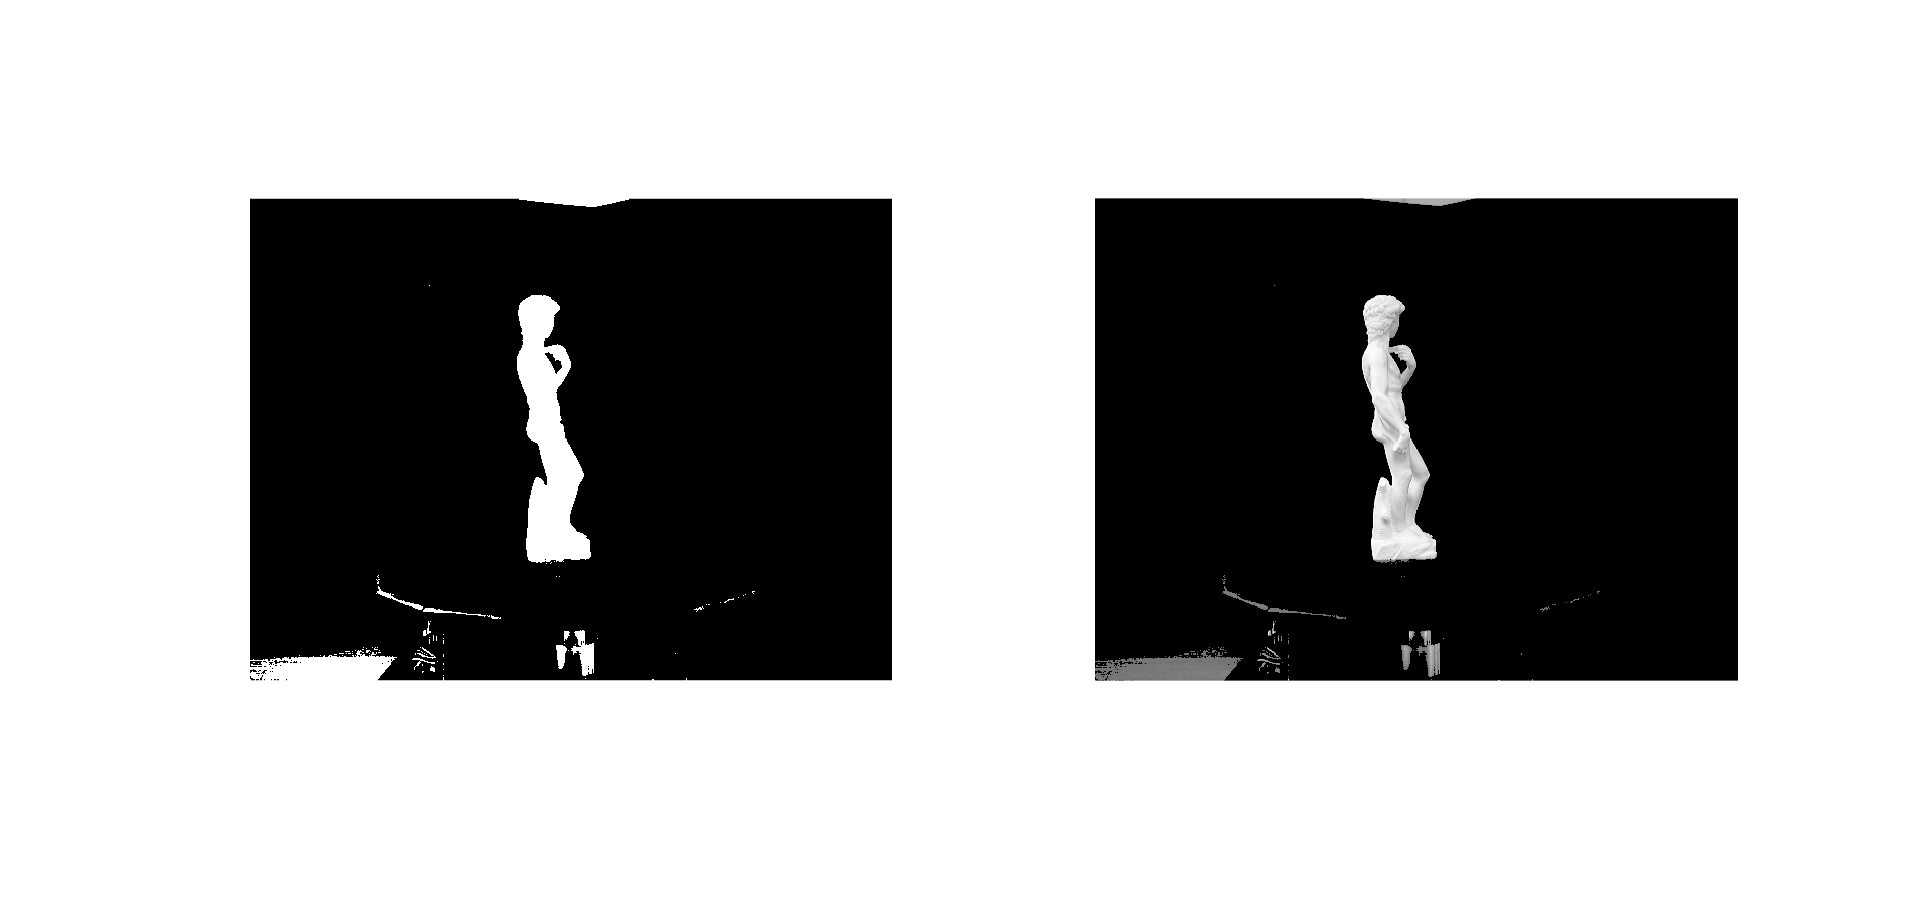
\includegraphics[width=1\linewidth, trim = {7cm 5cm 5cm 5cm}, clip]{C:/Users/Anton/Desktop/ETH_books/CV/cv_lab09_shape_from_silhouettes/code/results/untitled3}
			\end{minipage}
			
			\caption{Extracted silhouettes, threshold 110.}
		\end{center}
	\end{figure}

	\begin{figure}[h]
		\begin{center}
			\label{tang1}
			\begin{minipage}[h]{0.29\linewidth}
				\includegraphics[width=1\linewidth, trim = {6cm 4cm 6cm 3cm}, clip]{C:/Users/Anton/Desktop/ETH_books/CV/cv_lab09_shape_from_silhouettes/code/results/64-64-128/1}
			\end{minipage}
			\hfill
			\begin{minipage}[h]{0.29\linewidth}
				\includegraphics[width=1\linewidth, trim = {6cm 4cm 6cm 3cm}, clip]{C:/Users/Anton/Desktop/ETH_books/CV/cv_lab09_shape_from_silhouettes/code/results/64-64-128/2}
			\end{minipage}
				\hfill
				\begin{minipage}[h]{0.29\linewidth}
					\includegraphics[width=1\linewidth, trim = {6cm 4cm 6cm 3cm}, clip]{C:/Users/Anton/Desktop/ETH_books/CV/cv_lab09_shape_from_silhouettes/code/results/64-64-128/3}
			\end{minipage}

			
		\caption{3D-model screenshots, $64\times64\times128$.}
	\end{center}
\end{figure}
	\begin{figure}[h]
	\begin{center}
		\label{tang1}
		\begin{minipage}[h]{0.29\linewidth}
			\includegraphics[width=1\linewidth, trim = {6cm 4cm 6cm 3cm}, clip]{C:/Users/Anton/Desktop/ETH_books/CV/cv_lab09_shape_from_silhouettes/code/results/128-128-256/1}
		\end{minipage}
		\hfill
		\begin{minipage}[h]{0.29\linewidth}
			\includegraphics[width=1\linewidth, trim = {6cm 4cm 6cm 3cm}, clip]{C:/Users/Anton/Desktop/ETH_books/CV/cv_lab09_shape_from_silhouettes/code/results/128-128-256/2}
		\end{minipage}
		\hfill
		\begin{minipage}[h]{0.29\linewidth}
			\includegraphics[width=1\linewidth, trim = {6cm 4cm 6cm 3cm}, clip]{C:/Users/Anton/Desktop/ETH_books/CV/cv_lab09_shape_from_silhouettes/code/results/128-128-256/3}
		\end{minipage}
		
		\caption{3D-model screenshots, $128\times128\times256$. Model is better refined than with bounding box grid $64\times64\times128$, but also a little bit more <<noisy>> because of the inaccuracies in measurement and, probably, nature of the shape-from-voxels reconstructing algorithm.}
	\end{center}
\newpage
\textbf{Improvements}\\
Problems of the silhouette approach and possible ways to overcome them:
\begin{enumerate}
	\item to get well-refined model many images from different positions are needed
	\item resolution is determined by size of the used subboxes from the bounding box. This could be improved by iteratively using smaller meshgrid near the boundary of the object after obtaining the model at the coarser one (and checking now only these voxels, without checking those which are deep inside the object) 
	\item cavities in the object are hard to resolve. It could be done better if we detect some points of interest on several images from slightly different views and construct density map. So we will find, that cavity is farther than points nearby, and we will reconstruct it.
	\item it might be hard to get a silhouette of the object, especially when it's not of the uniform color. To overcome this points of interest, depth map or background detection (motion map) could be also used.
	\item the initial region of interest could be approximated better than a just box, if we use depth maps.
	\item when rotating for better accuracy object shouldn't be projected at the same place in image (so, here statue isn't in the center of the table for this purpose; otherwise, background pixels can be projected to the silhouette many times). It could be inconvenient in reality, when we don't have other choice 
	\item 3D--model can be constructed with true dimensions if we use known parameters of camera and/or if we make measurement with this special rotating table (then now distance between camera and object) 
	\item as an ultimate improvement, lidars could be used to scan surface of the object, but it would be less connected with computer vision (camera will be used inly for confirmation of the results from lidar + coloring of the model).
\end{enumerate}
\end{figure}

\end{document}
